\documentclass{ieeeaccess}
\usepackage{cite}
\usepackage{amsmath,amssymb,amsfonts}
\usepackage{graphicx}
\usepackage{textcomp}
\usepackage{booktabs}
\usepackage{multirow}
\usepackage{algorithm}
\usepackage{algorithmic}
\usepackage{url}
\usepackage[hidelinks]{hyperref}
\usepackage{xspace}

\newcommand{\abEtoEDiff}{0.63}
\newcommand{\abEtoEfour}{7.87}
\newcommand{\abEtoEzero}{7.23}
\newcommand{\abOverheadAuth}{0.102}
\newcommand{\abOverheadCache}{0.65}
\newcommand{\abOverheadFull}{0.75}
\newcommand{\abOverheadIn}{0.031}
\newcommand{\abOverheadOut}{0.596}
\newcommand{\abOverheadRbac}{0.017}
\newcommand{\awAbOverheadAuth}{0.045}
\newcommand{\awAbOverheadFull}{0.31}
\newcommand{\awBilled}{7}
\newcommand{\awBoundFracCacheMax}{116}
\newcommand{\awBoundFracMax}{105}
\newcommand{\awBoundFracMin}{93}
\newcommand{\awBreakeven}{606}
\newcommand{\awBreakevenFg}{343}
\newcommand{\awCNoneLat}{6.70}
\newcommand{\awCPropLat}{6.23}
\newcommand{\awCPropLatGain}{7.0}
\newcommand{\awCacheHitMax}{5.2}
\newcommand{\awCacheHitMin}{4.7}
\newcommand{\awCpuName}{Intel Xeon Platinum 8488C}
\newcommand{\awCpuTthree}{0.58}
\newcommand{\awCpuUnc}{0.249}
\newcommand{\awExtraRttSame}{1.0}
\newcommand{\awExtraRttSameTls}{9.5}
\newcommand{\awExtraRttXaz}{1.2}
\newcommand{\awExtraRttXazTls}{4.4}
\newcommand{\awExtraRttXreg}{1.0}
\newcommand{\awExtraRttXregTls}{2.1}
\newcommand{\awLevels}{128}
\newcommand{\awMapeMax}{5.4}
\newcommand{\awMapeMin}{0.5}
\newcommand{\awMapeOneMax}{33}
\newcommand{\awMapeOneMin}{0.5}
\newcommand{\awMapeRMax}{7}
\newcommand{\awMapeRMin}{1}
\newcommand{\awMidAuthMax}{0.035}
\newcommand{\awMidBig}{19.02}
\newcommand{\awMidDpiShareBig}{97}
\newcommand{\awMidPerKB}{74}
\newcommand{\awMidRbacMax}{0.005}
\newcommand{\awMidSmall}{0.19}
\newcommand{\awPython}{3.12.3}
\newcommand{\awRttSame}{0.15}
\newcommand{\awRttXaz}{0.53}
\newcommand{\awRttXreg}{12.7}
\newcommand{\awTfourPnnSame}{62}
\newcommand{\awTfourPnnSameTls}{63}
\newcommand{\awTfourPnnXaz}{65}
\newcommand{\awTfourPnnXazTls}{66}
\newcommand{\awTfourPnnXreg}{159}
\newcommand{\awTfourPnnXregTls}{166}
\newcommand{\awTfourSame}{6.96}
\newcommand{\awTfourSameTls}{7.13}
\newcommand{\awTfourXSame}{2508}
\newcommand{\awTfourXSameTls}{2496}
\newcommand{\awTfourXXaz}{2366}
\newcommand{\awTfourXXazTls}{2320}
\newcommand{\awTfourXXreg}{857}
\newcommand{\awTfourXXregTls}{825}
\newcommand{\awTfourXaz}{7.36}
\newcommand{\awTfourXazTls}{7.45}
\newcommand{\awTfourXreg}{19.31}
\newcommand{\awTfourXregTls}{19.13}
\newcommand{\awTlsCpuTthree}{1.58}
\newcommand{\awTlsPerCallSame}{1.40}
\newcommand{\awTthreeOverTfourSame}{1.02}
\newcommand{\awTthreeOverTfourSameTls}{1.19}
\newcommand{\awTthreeOverTfourXaz}{1.09}
\newcommand{\awTthreeOverTfourXazTls}{1.32}
\newcommand{\awTthreeOverTfourXreg}{1.68}
\newcommand{\awTthreeOverTfourXregTls}{2.40}
\newcommand{\awTthreeSame}{7.11}
\newcommand{\awTthreeSameTls}{8.51}
\newcommand{\awTthreeXSame}{2203}
\newcommand{\awTthreeXSameTls}{815}
\newcommand{\awTthreeXXaz}{2061}
\newcommand{\awTthreeXXazTls}{769}
\newcommand{\awTthreeXXreg}{513}
\newcommand{\awTthreeXXregTls}{347}
\newcommand{\awTthreeXaz}{8.02}
\newcommand{\awTthreeXazTls}{9.83}
\newcommand{\awTthreeXreg}{32.36}
\newcommand{\awTthreeXregTls}{46.00}
\newcommand{\awTtwoOverTfourInMax}{2.0}
\newcommand{\awTtwoOverTfourInMin}{1.8}
\newcommand{\awTtwoOverTfourXSame}{1.9}
\newcommand{\awTtwoOverTfourXSameTls}{1.8}
\newcommand{\awTtwoOverTfourXXaz}{2.0}
\newcommand{\awTtwoOverTfourXXazTls}{1.8}
\newcommand{\awTtwoOverTfourXXreg}{1.5}
\newcommand{\awTtwoOverTfourXXregTls}{1.5}
\newcommand{\awTtwoSame}{7.03}
\newcommand{\awTtwoSameTls}{7.13}
\newcommand{\awTtwoXSame}{4884}
\newcommand{\awTtwoXSameTls}{4552}
\newcommand{\awTtwoXXaz}{4619}
\newcommand{\awTtwoXXazTls}{4289}
\newcommand{\awTtwoXXreg}{1248}
\newcommand{\awTtwoXXregTls}{1254}
\newcommand{\awTtwoXaz}{7.42}
\newcommand{\awTtwoXazTls}{7.49}
\newcommand{\awTtwoXreg}{19.15}
\newcommand{\awTtwoXregTls}{19.63}
\newcommand{\cAlphaHi}{1.4}
\newcommand{\cGfifoHit}{31.9}
\newcommand{\cGfifoLat}{5.26}
\newcommand{\cGfifoLeak}{20.9}
\newcommand{\cGfifoSaved}{24.8}
\newcommand{\cGfifoStale}{10.8}
\newcommand{\cGlruHit}{31.9}
\newcommand{\cGlruHitHi}{42.8}
\newcommand{\cGlruLat}{5.31}
\newcommand{\cGlruLeak}{20.9}
\newcommand{\cGlruLeakHi}{29.9}
\newcommand{\cGlruSaved}{24.8}
\newcommand{\cGlruStale}{10.7}
\newcommand{\cNoneHit}{0.0}
\newcommand{\cNoneLat}{7.05}
\newcommand{\cNoneLeak}{0.0}
\newcommand{\cNoneSaved}{0.0}
\newcommand{\cNoneStale}{0.0}
\newcommand{\cPropHit}{9.3}
\newcommand{\cPropHitHi}{15.8}
\newcommand{\cPropLat}{6.55}
\newcommand{\cPropLatGain}{7.0}
\newcommand{\cPropLeak}{0.0}
\newcommand{\cPropSaved}{6.6}
\newcommand{\cPropSavedHi}{12.0}
\newcommand{\cPropStale}{0.0}
\newcommand{\cTlruHit}{13.0}
\newcommand{\cTlruLat}{6.43}
\newcommand{\cTlruLeak}{0.0}
\newcommand{\cTlruSaved}{9.5}
\newcommand{\cTlruStale}{4.0}
\newcommand{\cTttlHit}{9.6}
\newcommand{\cTttlLat}{6.52}
\newcommand{\cTttlLeak}{0.0}
\newcommand{\cTttlSaved}{6.7}
\newcommand{\cTttlSavedHi}{12.3}
\newcommand{\cTttlStale}{0.0}
\newcommand{\eCacheHit}{7.1}
\newcommand{\eTcacheRten}{17.56}
\newcommand{\eTcacheRtenPnn}{24.71}
\newcommand{\eTcacheRtwo}{9.89}
\newcommand{\eTcacheRtwoPnn}{16.22}
\newcommand{\eTcacheRzero}{7.18}
\newcommand{\eTcacheRzeroPnn}{13.10}
\newcommand{\eTfourRten}{18.72}
\newcommand{\eTfourRtenPnn}{24.71}
\newcommand{\eTfourRtwo}{10.52}
\newcommand{\eTfourRtwoPnn}{16.35}
\newcommand{\eTfourRzero}{7.55}
\newcommand{\eTfourRzeroPnn}{13.00}
\newcommand{\eToneRzero}{7.16}
\newcommand{\eToneRzeroPnn}{12.77}
\newcommand{\eTthreeMinusTfourRten}{21.75}
\newcommand{\eTthreeMinusTfourRzero}{0.79}
\newcommand{\eTthreeOverTfourRten}{2.16}
\newcommand{\eTthreeOverTfourRtwo}{1.53}
\newcommand{\eTthreeRten}{40.47}
\newcommand{\eTthreeRtenPnn}{46.47}
\newcommand{\eTthreeRtwo}{16.07}
\newcommand{\eTthreeRtwoPnn}{21.87}
\newcommand{\eTthreeRzero}{8.33}
\newcommand{\eTthreeRzeroPnn}{14.24}
\newcommand{\eTtwoRten}{18.73}
\newcommand{\eTtwoRtenPnn}{24.44}
\newcommand{\eTtwoRtwo}{10.55}
\newcommand{\eTtwoRtwoPnn}{16.47}
\newcommand{\eTtwoRzero}{7.70}
\newcommand{\eTtwoRzeroPnn}{13.25}
\newcommand{\extAttacks}{2,371}
\newcommand{\extAttacksDetected}{0}
\newcommand{\extBenign}{738}
\newcommand{\extBenignFp}{0}
\newcommand{\extDsBen}{399}
\newcommand{\extDsDetected}{0}
\newcommand{\extDsFp}{0}
\newcommand{\extDsMal}{263}
\newcommand{\extIaAllBlocked}{0}
\newcommand{\extIaBase}{1,054}
\newcommand{\extIaBlocked}{0}
\newcommand{\extIaEnh}{1,054}
\newcommand{\extIaN}{2,108}
\newcommand{\extNiFp}{0}
\newcommand{\extNiN}{339}
\newcommand{\hBilled}{101}
\newcommand{\hBreakeven}{150}
\newcommand{\hBreakevenFg}{85}
\newcommand{\hCPropLatGain}{6.9}
\newcommand{\hCPropSavedMs}{6.1}
\newcommand{\hMapeMax}{5.3}
\newcommand{\hMapeMin}{1.8}
\newcommand{\hMapeOneMax}{7.1}
\newcommand{\hToolMax}{181}
\newcommand{\hToolMean}{101}
\newcommand{\hToolMin}{35}
\newcommand{\hTthreeMinusTfourRten}{21.7}
\newcommand{\hTthreeOverTfourRten}{1.20}
\newcommand{\igMabl}{0.087}
\newcommand{\igMmid}{0.066}
\newcommand{\igMone}{0.038}
\newcommand{\kAlb}{16.43}
\newcommand{\kBeFgHundred}{84}
\newcommand{\kBeFgTen}{287}
\newcommand{\kBeFgThousand}{10}
\newcommand{\kBeHundred}{148}
\newcommand{\kBeTen}{508}
\newcommand{\kBeThousand}{18}
\newcommand{\kBilled}{11}
\newcommand{\kBreakeven}{537}
\newcommand{\kBreakevenFg}{303}
\newcommand{\kCapVcpu}{4.2}
\newcommand{\kCpuC}{0.351}
\newcommand{\kCpuUnc}{0.371}
\newcommand{\kDfourThousand}{157}
\newcommand{\kDoneThousand}{292}
\newcommand{\kEcTwo}{70.08}
\newcommand{\kEcTwoMin}{157}
\newcommand{\kFargate}{36.04}
\newcommand{\kFargateMin}{89}
\newcommand{\kGwSide}{0.48}
\newcommand{\kHit}{9.3}
\newcommand{\kHitAtThirtyTwo}{10}
\newcommand{\kHitConc}{4.8}
\newcommand{\kLamHundred}{1.06}
\newcommand{\kLamTen}{0.31}
\newcommand{\kLamThousand}{8.56}
\newcommand{\kUtil}{60}
\newcommand{\kVcpuShareThousand}{14}
\newcommand{\mAuthMax}{0.067}
\newcommand{\mBigKB}{31.6}
\newcommand{\mBigSize}{256}
\newcommand{\mDpiShareBig}{97}
\newcommand{\mOneKB}{0.32}
\newcommand{\mPerKB}{123}
\newcommand{\mRbacMax}{0.011}
\newcommand{\qBoundFracMax}{98}
\newcommand{\qBoundFracMin}{84}
\newcommand{\qHeapMaxAll}{2.6}
\newcommand{\qMapeRMax}{7}
\newcommand{\qMapeRMin}{4}
\newcommand{\qMapeROneMax}{101}
\newcommand{\qMapeROneMin}{24}
\newcommand{\qMapeXMax}{10}
\newcommand{\qMapeXMin}{6}
\newcommand{\qMapeXOneMax}{33}
\newcommand{\qMapeXOneMin}{15}
\newcommand{\qPool}{16}
\newcommand{\qRtt}{2}
\newcommand{\qTcacheDcpumax}{0.42}
\newcommand{\qTcacheDcpuone}{1.12}
\newcommand{\qTcacheGain}{9}
\newcommand{\qTcacheHeapmax}{2.2}
\newcommand{\qTcacheHitMax}{4.8}
\newcommand{\qTcacheHitOne}{12.6}
\newcommand{\qTcacheHold}{9.97}
\newcommand{\qTcacheKnee}{15}
\newcommand{\qTcacheMapeR}{4}
\newcommand{\qTcacheMapeRone}{37}
\newcommand{\qTcacheMapeX}{6}
\newcommand{\qTcacheMapeXone}{21}
\newcommand{\qTcachePnnmax}{107}
\newcommand{\qTcacheXmax}{1578}
\newcommand{\qTfourBound}{1644}
\newcommand{\qTfourDcpumax}{0.42}
\newcommand{\qTfourDcpuone}{1.03}
\newcommand{\qTfourHeapmax}{1.6}
\newcommand{\qTfourHold}{9.73}
\newcommand{\qTfourKnee}{17}
\newcommand{\qTfourMapeR}{6}
\newcommand{\qTfourMapeRone}{24}
\newcommand{\qTfourMapeX}{8}
\newcommand{\qTfourMapeXone}{15}
\newcommand{\qTfourMeanmax}{91}
\newcommand{\qTfourOverTthree}{1.6}
\newcommand{\qTfourPnnmax}{107}
\newcommand{\qTfourXmax}{1451}
\newcommand{\qTthreeBound}{1030}
\newcommand{\qTthreeDcpumax}{0.76}
\newcommand{\qTthreeDcpuone}{2.60}
\newcommand{\qTthreeHeapmax}{2.6}
\newcommand{\qTthreeHold}{15.53}
\newcommand{\qTthreeKnee}{17}
\newcommand{\qTthreeMapeR}{7}
\newcommand{\qTthreeMapeRone}{68}
\newcommand{\qTthreeMapeX}{10}
\newcommand{\qTthreeMapeXone}{31}
\newcommand{\qTthreePnnmax}{165}
\newcommand{\qTthreeXmax}{890}
\newcommand{\qTtwoCpuBound}{2849}
\newcommand{\qTtwoDcpumax}{0.35}
\newcommand{\qTtwoDcpuone}{1.37}
\newcommand{\qTtwoHeapmax}{1.6}
\newcommand{\qTtwoHold}{3.41}
\newcommand{\qTtwoKnee}{30}
\newcommand{\qTtwoMapeR}{7}
\newcommand{\qTtwoMapeRone}{101}
\newcommand{\qTtwoMapeX}{9}
\newcommand{\qTtwoMapeXone}{33}
\newcommand{\qTtwoMeanmax}{53}
\newcommand{\qTtwoOverTthree}{2.7}
\newcommand{\qTtwoPnnmax}{64}
\newcommand{\qTtwoXmax}{2392}
\newcommand{\sTfourRten}{21.3}
\newcommand{\sTfourRzero}{0.29}
\newcommand{\sTone}{296}
\newcommand{\sTtwoRten}{33.9}
\newcommand{\sTtwoRzero}{1.28}
\newcommand{\secBen}{170}
\newcommand{\secEva}{0.0}
\newcommand{\secFPR}{17.6}
\newcommand{\secMal}{240}
\newcommand{\secOrdFP}{0}
\newcommand{\secPrecision}{84.2}
\newcommand{\secRecall}{66.7}
\newcommand{\secSig}{100.0}
\newcommand{\secVocabFP}{100}
\newcommand{\senBonf}{0.0083}
\newcommand{\senCapB}{256}
\newcommand{\senCapM}{64}
\newcommand{\senCapS}{16}
\newcommand{\senCurHi}{34}
\newcommand{\senCurLo}{8}
\newcommand{\senEvictCells}{6}
\newcommand{\senGainCur}{0.4}
\newcommand{\senGainMod}{1.0}
\newcommand{\senGainWide}{1.6}
\newcommand{\senHitLoss}{0.2}
\newcommand{\senLossMax}{0.23}
\newcommand{\senLossMin}{0.15}
\newcommand{\senPCur}{$p = 0.03$}
\newcommand{\senPMidMax}{$p = 0.02$}
\newcommand{\senPMod}{$p = 0.001$}
\newcommand{\senPWide}{$p < 0.001$}
\newcommand{\senRelCur}{10}
\newcommand{\senRelMod}{27}
\newcommand{\senRelWide}{41}
\newcommand{\senSeeds}{20}
\newcommand{\senTrace}{400}
\newcommand{\tbIoScale}{0.25}
\newcommand{\tbPython}{3.14.0}
\newcommand{\wcCraftedBig}{24.7\,s}
\newcommand{\wcCraftedMid}{1.6\,s}
\newcommand{\wcCraftedSmall}{97\ms}
\newcommand{\wcKbBig}{256}
\newcommand{\wcKbMid}{64}
\newcommand{\wcKbSmall}{16}


\newcommand{\ms}{\,ms\xspace}

\makeatletter
\AtBeginDocument{\DeclareMathVersion{bold}
\SetSymbolFont{operators}{bold}{T1}{times}{b}{n}
\SetSymbolFont{NewLetters}{bold}{T1}{times}{b}{it}
\SetMathAlphabet{\mathrm}{bold}{T1}{times}{b}{n}
\SetMathAlphabet{\mathit}{bold}{T1}{times}{b}{it}
\SetMathAlphabet{\mathbf}{bold}{T1}{times}{b}{n}
\SetMathAlphabet{\mathtt}{bold}{OT1}{pcr}{b}{n}
\SetSymbolFont{symbols}{bold}{OMS}{cmsy}{b}{n}
\renewcommand\boldmath{\@nomath\boldmath\mathversion{bold}}}
\makeatother

\begin{document}
\history{Date of publication xxxx 00, 0000, date of current version xxxx 00, 0000.}
\doi{10.1109/ACCESS.2024.0429000}

\title{Transport, Policy, and Caching Trade-offs in Security-Enforcing Gateways for the Model Context Protocol: An Empirical Study}

\author{\uppercase{He Li}\authorrefmark{1,*} and \uppercase{Yi Zhong}\authorrefmark{2,*}}

\address[1]{Cornell University, Ithaca, NY, USA (e-mail: hl746@cornell.edu)}
\address[2]{Columbia University, New York, NY, USA (e-mail: yz3935@columbia.edu)}
\address[*]{These authors contributed equally to this work.}

\markboth
{H. Li and Y. Zhong: Security-Enforcing Gateways for the Model Context Protocol}
{H. Li and Y. Zhong: Security-Enforcing Gateways for the Model Context Protocol}

\corresp{Corresponding author: Yi Zhong (e-mail: yz3935@columbia.edu).}

\begin{abstract}
Large language model agents increasingly call enterprise tools through the Model Context Protocol (MCP), often via a gateway that centralizes security and caching, whose costs have rarely been measured. We build an MCP gateway with identity, authorization, inspection, and caching stages and four upstream transports, and evaluate it on one host with emulated network delay and on Amazon EC2 at three network distances over TCP and TLS~1.3. First, connection reuse dominates transport cost on real networks: across regions with TLS, unpooled Streamable HTTP is \awTthreeOverTfourXregTls$\times$ slower per call than pooled, and per-call TLS handshakes more than halve unpooled capacity even within one zone. Second, identity and authorization checks cost about 0.1\ms per call and stop every credential and authorization violation tested, whereas signature-based inspection is the only stage whose cost grows with payload size, reaching \mDpiShareBig\% of gateway time at \mBigSize\,KB, yet it detects none of \extAttacks\ attacks from public prompt-injection datasets. Third, caches that ignore the tenant achieve the highest hit rates but answer \cGlruLeak\% of calls with another tenant's data; tenant-scoped keys with per-tool freshness bounds eliminate leaked and stale responses at the cost of hit rate. A queueing bound matches maximum throughput on EC2 within \awMapeMin--\awMapeMax\% with CPU cost measured under load (\awMapeOneMin--\awMapeOneMax\% with single-session measurements), and a cost model shows that because serverless billing includes time spent waiting on tools, its cost advantage disappears at lower volumes as tool latency grows.
\end{abstract}

\begin{keywords}
API gateway, cloud cost, large language model agents, Model Context Protocol, multi-tenant caching, performance evaluation, prompt injection, queueing model, tool calling.
\end{keywords}

\titlepgskip=-21pt

\maketitle

% =====================================================================================
\section{Introduction}
\label{sec:intro}

\IEEEPARstart{L}{arge} language model (LLM) agents act on the world by calling tools that retrieve documents, query databases, and trigger deployments~\cite{schick2023toolformer,yao2023react,qin2024toolllm,patil2024gorilla}. The Model Context Protocol (MCP)~\cite{anthropic2024mcp} standardizes this interaction as JSON-RPC messages exchanged between an agent-side client and a tool-hosting server, over either a local stdio pipe or HTTP~\cite{mcpspec20241105,mcpspec20250326,mcpspec20260728}. When dozens of MCP servers serve many agents and tenants, implementing authentication, least privilege, injection defenses, and data protection separately in each server is error-prone. The industry response is the \emph{MCP gateway}, a proxy that terminates agent connections, applies security policy in one place, and forwards calls to upstream servers~\cite{brett2025simplified,narajala2025enterprise,errico2025securing,kumar2026gateway,li2026zerotrust}.

Existing work on MCP gateways describes architectures, threat models, and authentication designs, and the few measurements~\cite{ahmadi2025mcpbridge,li2026mcpgateway} do not isolate what the gateway's security, transport, caching, and deployment choices cost: which upstream transport to use and whether to pool connections, which security stages to enable, how to cache tool results across tenants, and whether to deploy on serverless functions, containers, or virtual machines. We measure these costs with a gateway prototype whose upstream MCP server runs in a separate process reached over real pipes or sockets, with only the tool service time and, where stated, the network round-trip time (RTT) emulated, and repeat the transport and concurrency experiments on Amazon EC2 across zones and regions over TCP and TLS~1.3. Every experiment runs five independent trials (three for the concurrency sweeps). The contributions are:
\begin{enumerate}
\item A gateway design with identity and delegation (M1), per-tool authorization (M2), bidirectional inspection (M3), and a tenant-scoped, freshness-bounded, cost-aware cache (M4) (Section~\ref{sec:design}).
\item A transport comparison across stdio, legacy HTTP+\allowbreak SSE, and Streamable HTTP with and without pooling, at loopback and emulated 2\ms and 10\ms RTTs, validated on EC2 at three network distances (\awRttSame--\awRttXreg\ms RTT) with and without TLS~1.3 (Sections~\ref{sec:res-transport} and~\ref{sec:res-concurrency}).
\item A per-stage cost breakdown for payloads of 1 to \mBigSize\,KB, and an ablation that measures what each stage's latency buys in detection on a 410-case suite with known-signature and evasive subsets and on \extAttacks\ attacks and \extBenign\ benign prompts from three public datasets (Sections~\ref{sec:res-middleware}--\ref{sec:res-security}).
\item A comparison of six cache policies trading hit rate against cross-tenant leakage and staleness (Section~\ref{sec:res-cache}).
\item A queueing bound validated against 1 to 128 concurrent sessions on one host and on EC2, and a cloud cost model driven by measured CPU time and latency (Sections~\ref{sec:model}, \ref{sec:res-concurrency}--\ref{sec:res-cost}).
\end{enumerate}

We report negative results alongside positive ones: our deliberately minimal signature inspection is the most expensive security stage yet buys the least protection, and correct caching costs hit rate.

% =====================================================================================
\section{Background and Related Work}
\label{sec:related}

\subsection{The Model Context Protocol and Its Transports}
MCP~\cite{anthropic2024mcp} defines JSON-RPC 2.0 messages for capability negotiation (\texttt{initialize}), tool discovery (\texttt{tools/list}), and invocation (\texttt{tools/call}), among others. The \emph{stdio} transport runs the server as a child process of the client, tying one server process to one client. In the \emph{HTTP with server-sent events} (HTTP+SSE) transport of revision 2024-11-05~\cite{mcpspec20241105}, requests are POSTed to a per-session endpoint, acknowledged with \texttt{202 Accepted}, and answered on a long-lived event stream, so the server holds per-session state. Revision 2025-03-26~\cite{mcpspec20250326} replaced it with \emph{Streamable HTTP}, in which each request is a POST answered in the response body, and revision 2026-07-28~\cite{mcpspec20260728} removed protocol-level sessions. Streamable HTTP leaves connection management to the HTTP layer, so a gateway may connect per call or reuse persistent connections~\cite{mogul1995persistent,rfc9112}; we evaluate both because scale-to-zero deployments often cannot keep pools warm.

\subsection{MCP Security and Gateways}
Hou et al.~\cite{hou2025mcp} survey MCP threats; guidance recommends tool-poisoning defenses~\cite{narajala2025enterprise}, per-user authentication, scoped authorization, inline data-loss prevention (DLP), and centralized gateways~\cite{errico2025securing,brett2025simplified}. Kumar et al.~\cite{kumar2026gateway} separate user and non-user personas so that automation cannot impersonate humans, a boundary our M1 stage enforces. Li et al.~\cite{li2026zerotrust} show that per-tool authorization must be enforced at invocation time, because hiding a tool from discovery does not stop clients or models from calling it. MCP-connected LLMs can be coerced into code execution and credential theft~\cite{radosevich2025audit}, and existing protections stop fewer than 30\% of attacks on average~\cite{yang2025mcpsecbench}. A REST proxy for MCP adds 1.07--1.64\ms per call~\cite{ahmadi2025mcpbridge}, and long-lived backend connections cut a production gateway's mean and P99 latency by 51.7\% and 56.5\%~\cite{li2026mcpgateway}, consistent with our pooling results; neither measures security stages, TLS, tenant-scoped caching, or deployment cost.

\subsection{Prompt Injection}
Indirect prompt injection, in which instructions hidden in tool output steer an agent~\cite{greshake2023not}, tops OWASP's LLM risks~\cite{owasp2025llm} and is benchmarked by InjecAgent~\cite{zhan2024injecagent}, AgentDojo~\cite{debenedetti2024agentdojo}, and Liu et al.~\cite{liu2024formalizing}. These studies find detection-based defenses fragile. Learned detectors cost far more per input, from about 15\ms for a lightweight prompt-guard classifier to seconds for GPT-4o~\cite{li2024injecguard} or a fine-tuned LLM~\cite{liu2025datasentinel}, and over-defend, flagging benign inputs that contain trigger words such as ``ignore''~\cite{li2024injecguard}. Our inspection stage is deliberately a minimal signature detector of five regular-expression rule groups, cheap and predictable with easily attributed failures; larger rule sets would still match wording rather than intent, and we do not evaluate learned detectors.

\subsection{Gateways, Caching, and Performance Modeling}
Service-mesh sidecars~\cite{li2019servicemesh} can raise latency by up to 269\% and CPU use by up to 163\%, dominated by HTTP-layer parsing~\cite{zhu2023dissecting}. Zero-trust architectures authorize every request~\cite{rose2020zerotrust,ward2014beyondcorp}. Web proxy caching under Zipf-like popularity~\cite{breslau1999zipf} and cost-aware replacement~\cite{cao1997cost} are classical, and semantic caches such as GPTCache~\cite{bang2023gptcache} cache LLM responses. Tool results differ from web objects in being authorization-dependent and having tool-specific freshness requirements. We use asymptotic bound analysis and Little's law~\cite{lazowska1984qsp,little1961proof} for capacity, and the serverless literature~\cite{jonas2019cloud,wang2018peeking} for deployment trade-offs.

% =====================================================================================
\section{Threat Model and Requirements}
\label{sec:threat}

\emph{Assets} are the data and actions exposed by upstream tools: documents, analytics, infrastructure telemetry, and mutating operations such as privilege grants and deployments. \emph{Principals} are interactive users, agents acting on behalf of users through delegation, and headless services; each belongs to a tenant. We consider four adversaries: (A1) an external caller presenting a missing, forged, expired, or tampered credential; (A2) an authenticated caller, possibly a prompt-injected agent, requesting a tool or argument outside its authority, including a service principal claiming to act for a human; (A3) attacker-controlled text inside tool arguments (injected instructions, server-side request forgery targets, command or SQL fragments); and (A4) a compromised or malicious upstream server that returns instructions aimed at the agent (tool poisoning) or leaks secrets and personal data. A fifth risk arises from the gateway itself: a shared cache may serve one tenant's authorization-dependent result to another, or serve a result older than the tool's freshness requirement.

The gateway must therefore (R1) verify every call's credential and enforce the persona boundary on delegation chains~\cite{kumar2026gateway,jones2020rfc8693,hardy1988confused}; (R2) authorize each call per tool and validate arguments against the tool's input schema~\cite{li2026zerotrust}; (R3) block arguments that carry injected instructions or attack payloads and responses that carry poisoning, and redact secrets and personal data from responses; (R4) never answer a call with data produced for another tenant or older than the tool's freshness bound; and (R5) impose a per-call latency and CPU cost that is measured for each control and justified by the attacks that control stops. The security conformance suite (Section~\ref{sec:method}) tests each adversary: category C1 targets A1 and the delegation abuse in A2, C2 the remainder of A2, C3 and C4 target A3, and C5 and C6 target A4, while the cache experiments (Section~\ref{sec:res-cache}) test R4. We do not address compromise of the gateway host or attacks that succeed entirely within the agent without a tool call. We also do not address denial of service. The ordering of stages means unauthenticated floods are rejected at M1 for about 0.1\ms each, but the prototype has no per-tenant rate limit or payload-size cap, and because inspection cost grows linearly with payload size, an authenticated caller sending large payloads can consume disproportionate gateway CPU, and a single crafted upstream response can stall the gateway for seconds (Section~\ref{sec:res-middleware}). Production deployments would add per-tenant rate limits and payload-size limits ahead of M3, and rely on network-layer protection against volumetric attacks.

% =====================================================================================
\section{Gateway Design}
\label{sec:design}

Fig.~\ref{fig:arch} shows the gateway. Each call passes through four stages; a call is rejected at the first stage that fails, and a cache hit returns before any upstream I/O.

\begin{figure}[t]
\centering
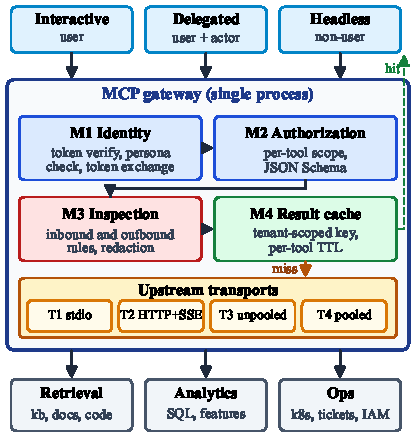
\includegraphics[width=\columnwidth]{figures/fig1_architecture.pdf}
\caption{Gateway architecture. Callers of three personas reach a single gateway process that applies identity (M1), authorization (M2), inspection (M3), and caching (M4) before forwarding misses over one of four upstream transports.}
\label{fig:arch}
\end{figure}

\subsection{M1: Identity and Delegation}
Callers present a signed bearer token (HMAC-SHA-256 in the prototype; a JWT verifier in production) whose claims carry the subject, persona $\in\{\text{user}, \text{non\_user}\}$, scopes, tenant, expiry, and an optional actor claim \texttt{act} in the style of OAuth~2.0 Token Exchange~\cite{jones2020rfc8693}. M1 verifies the signature and expiry, then enforces the persona boundary: a non-user principal may not present an actor chain that names a user persona, because no user-consented exchange could have produced it~\cite{kumar2026gateway}. This rejects the confused-deputy pattern~\cite{hardy1988confused} in which a service account claims to act for a human. M1 then mints a downstream delegation token scoped to the upstream audience. The authenticated tenant is forwarded upstream in the request's \texttt{\_meta} field so that upstream servers can apply their own authorization.

\subsection{M2: Per-Tool Authorization and Schema Validation}
Each tool declares a required scope and a JSON input schema. M2 rejects calls to unknown tools, calls without the required scope, calls by non-user principals to tools reserved for interactive users (here, just-in-time privilege grants), and arguments that omit required fields or have the wrong type. Enforcement happens at invocation time, independent of what the agent was shown during discovery~\cite{li2026zerotrust}.

\subsection{M3: Bidirectional Inspection}
Inbound, M3 serializes the call parameters and matches them against signature rules for injected directives, poisoning markup, path traversal and cloud metadata endpoints, shell and SQL fragments, and known exfiltration endpoints. Outbound, it blocks responses containing poisoning markup and redacts AWS access keys, API secrets, US social security numbers, and e-mail addresses. Both directions are linear-time scans over the serialized payload.

\subsection{M4: Tenant-Scoped, Freshness-Bounded Cache}
Only tools that declare themselves cacheable (read-only) are cached. For a call by tenant $t$ with persona $p$ to tool $f$ with arguments $a$, the cache key is
\begin{equation}
k = (t,\; p,\; f,\; \mathrm{SHA256}(\mathrm{canon}(a))),
\label{eq:key}
\end{equation}
where $\mathrm{canon}$ serializes arguments with sorted keys and the prototype keeps the first 96 bits of the hash. Tool-discovery (\texttt{tools/list}) results are also cached, under the key $(t, p)$. Including $t$ and $p$ guarantees that an authorization-dependent result is returned only to callers in the same tenant and persona (R4). An entry inserted at time $s$ expires at $s + \tau_f$, where $\tau_f$ is the freshness bound declared in the tool's metadata (in our upstream server, illustrative values that we set: 15--30\,s for pod telemetry and error-budget burn rates, 60--120\,s for features and analytics, 300--600\,s for documents and cost roll-ups), so no response older than $\tau_f$ is served. When the cache is full, the proposed policy examines the $w = 4$ least recently used entries and evicts the one whose tool has the lowest expected upstream cost $c_f$, a windowed variant of cost-aware replacement~\cite{cao1997cost} that keeps expensive results longer at the price of a slightly less recency-faithful order. In our measurements this pays off only when the cache is small relative to the working set and tool costs differ widely; at larger capacities plain LRU is as good or slightly better (Section~\ref{sec:res-cache}). Algorithm~\ref{alg:pipeline} summarizes the pipeline.

\begin{algorithm}[t]
\caption{Gateway request pipeline}
\label{alg:pipeline}
\begin{algorithmic}[1]
\REQUIRE token $\theta$, JSON-RPC call $(f, a)$, transport $T$
\STATE $(ok, \kappa) \gets \textsc{VerifyAndExchange}(\theta)$ \COMMENT{M1}
\IF{$\neg ok$ \OR ($\kappa.\mathit{persona}=\text{non\_user} \wedge \kappa.\mathit{act.persona}=\text{user}$)} \RETURN error \ENDIF
\IF{$\neg\textsc{Authorized}(\kappa, f) \vee \neg\textsc{SchemaValid}(f, a)$} \RETURN error \COMMENT{M2} \ENDIF
\IF{$\textsc{InboundRuleMatch}(f, a)$} \RETURN error \COMMENT{M3-in} \ENDIF
\STATE $k \gets (\kappa.t, \kappa.p, f, \mathrm{SHA256}(\mathrm{canon}(a)))$ \COMMENT{M4}
\IF{$k \in \mathcal{C}$ \AND $\mathit{now} \le \mathcal{C}[k].s + \tau_f$} \RETURN $\mathcal{C}[k].r$ \ENDIF
\STATE $r \gets T.\textsc{Send}(f, a, \kappa.t)$
\IF{$\textsc{OutboundPoisoned}(r)$} \RETURN error \COMMENT{M3-out} \ENDIF
\STATE $r \gets \textsc{Redact}(r)$
\IF{$f$ cacheable} \STATE $\textsc{Insert}(\mathcal{C}, k, r, \mathit{now})$ \COMMENT{cost-aware eviction} \ENDIF
\RETURN $r$
\end{algorithmic}
\end{algorithm}

\subsection{Upstream Transports}
The prototype implements four transports to the same upstream server code: \textbf{T1} keeps a persistent stdio child process; \textbf{T2} implements the 2024-11-05 HTTP+SSE transport with one event stream per gateway session and a pool of persistent POST connections; \textbf{T3} implements Streamable HTTP with a new TCP connection per call (\texttt{Connection: close}), as in a stateless or scale-to-zero deployment; and \textbf{T4} implements Streamable HTTP over a fixed pool of $c$ persistent keep-alive connections shared by all agent sessions. T3 and T4 hold one of $c$ connections for the whole call, so they bound in-flight calls to $c$. T2 also uses $c$ POST connections, but holds one only until the \texttt{202 Accepted} acknowledgment and receives the response on the event stream, so it bounds concurrent request submissions rather than in-flight calls.

% =====================================================================================
\section{Performance and Cost Models}
\label{sec:model}

\subsection{Asymptotic Bounds for Concurrent Sessions}
We model $N$ agent sessions that each issue calls back to back (a closed system with zero think time). Let $R_1$ be the response time of an isolated call, $D_{\mathrm{cpu}}$ the CPU time the gateway process spends per call (the prototype runs a single event loop, so CPU is a single-server station), and $S_{\mathrm{hold}}$ the time a call occupies one of the $c$ connections (a $c$-server station). Asymptotic bound analysis~\cite{lazowska1984qsp} gives the throughput bound
\begin{equation}
X(N) \le \min\!\left(\frac{N}{R_1},\; \frac{1}{D_{\mathrm{cpu}}},\; \frac{c}{S_{\mathrm{hold}}}\right),
\label{eq:aba}
\end{equation}
and Little's law~\cite{little1961proof} gives the corresponding response time $R(N) = N / X(N)$. The bottleneck is the station with the largest per-call demand, $D_{\max} = \max(D_{\mathrm{cpu}}, S_{\mathrm{hold}}/c)$, and the knee beyond which queueing dominates is $N^* = R_1 / D_{\max}$. Because the bound ignores queueing among calls with variable service times, measured throughput lies below it, most visibly near the knee $N^*$; the bound's value is in identifying the bottleneck and its asymptote, not in predicting throughput exactly.

We measure $R_1$ and $S_{\mathrm{hold}}$ at $N=1$, and $D_{\mathrm{cpu}}$ from process CPU accounting. Because the load generator runs in the gateway's process, $D_{\mathrm{cpu}}$ includes the cost of generating load and therefore overstates the gateway's own CPU cost. CPU time per call also falls as load rises (Section~\ref{sec:res-concurrency}), so we evaluate the model twice: with $D_{\mathrm{cpu}}$ measured at $N=1$, which uses no measurement under load, and with $D_{\mathrm{cpu}}$ measured at the largest $N$, which is taken from the CPU accounting of the same runs whose throughput is predicted.

For an unpooled transport, each call opens a connection, so $S_{\mathrm{hold}}$ includes one extra RTT for the TCP handshake and, with TLS~1.3, a second for the TLS handshake~\cite{rfc8446}, in addition to the request RTT and service time; for a pooled transport, it includes only the request RTT and service time. Equation~\eqref{eq:aba} therefore predicts that pooling raises the connection-bound capacity by a factor of $(S + 3\,\mathrm{RTT})/(S + \mathrm{RTT})$ with TLS and $(S + 2\,\mathrm{RTT})/(S + \mathrm{RTT})$ without, for service time $S$. The emulated-delay experiments charge both handshakes on every new connection and so correspond to the TLS case.

\subsection{Deployment Cost}
For monthly call volume $V$ (millions), a serverless deployment billed per request and per GB-second costs
\begin{equation}
C_{\lambda}(V) = V\,(p_{\mathrm{req}} + 10^{6} \cdot \lceil d \rceil_{\mathrm{ms}} \cdot m \cdot p_{\mathrm{GBs}}),
\label{eq:lambda}
\end{equation}
where $d$ is the billed duration in seconds, rounded up to the next millisecond, and $m$ the memory size in GB. Because serverless functions are billed for wall-clock time, $d$ includes the time spent waiting for the upstream tool. An always-on deployment with replicas of $v$ vCPUs, a monthly replica price $p_{\mathrm{vm}}$, a minimum of $n_{\min}$ replicas, a target CPU utilization $u$, and a load balancer at $p_{\mathrm{lb}}$ per month costs
\begin{equation}
C_{\mathrm{vm}}(V) = p_{\mathrm{vm}} \max\!\left(n_{\min}, \left\lceil \frac{10^6\, V\, D_{\mathrm{cpu}}}{u \cdot v \cdot 2.628\times 10^{6}\,\mathrm{s}} \right\rceil\right) + p_{\mathrm{lb}}.
\label{eq:vm}
\end{equation}
Since $D_{\mathrm{cpu}}$ is measured per call, the replica count, and therefore the break-even volume where $C_\lambda(V) = C_{\mathrm{vm}}(V)$, follows from measurements rather than assumed capacities. Equation~\eqref{eq:vm} assumes that a replica runs one event loop per vCPU, whereas the prototype runs one in total. Equation~\eqref{eq:lambda} assumes warm function instances that each serve one request at a time and does not model cold starts.

% =====================================================================================
\section{Experimental Methodology}
\label{sec:method}

\subsection{Testbed}
Every experiment runs on a single host (Intel Core i7-14700HX, 20 cores and 28 threads, 32\,GB RAM, Windows 11, CPython \tbPython) and is repeated on Amazon EC2 (Section~\ref{sec:method-aws}): all experiments in one availability zone over TCP, and the transport and concurrency experiments at all three placements, over both TCP and TLS~1.3. The load generator and gateway share one process and one asyncio event loop; the upstream MCP server runs in a separate process, reached over stdin/stdout pipes (T1) or loopback TCP with HTTP/1.1 framing (T2--T4). The connection pools of T2 and T4 hand each returned connection to the longest-waiting call, so no session is starved under saturation. The default Windows timer tick of 15.6\ms quantizes \texttt{asyncio.sleep}; in a calibration run, a 1.8\ms sleep took 15.5\ms (median) by default and 2.7\ms with 1\ms timer resolution. Every process in the testbed therefore requests 1\ms resolution, without which sub-tick latency differences would be invisible.

\subsection{Multi-Host Testbed on Amazon EC2}
\label{sec:method-aws}
For the multi-host validation, the gateway (with the load generator, as above) and the upstream server run on two \texttt{c7i.large} instances (2 vCPUs of an \awCpuName, 4\,GB RAM, Ubuntu 24.04, CPython \awPython). A small control agent on the upstream instance starts an upstream server per experiment, so the harness is unchanged. We use three placements: both instances in us-east-1a; the upstream in us-east-1b; and the upstream in us-east-2a (Ohio), reached over its public address. RTT is measured as the median of 200 TCP connection setups between the instances. No delay is emulated. Each placement runs over plain TCP and over TLS~1.3 (ECDHE with a P-256 certificate, a full handshake per new connection and no session resumption); the client does not verify the self-signed certificate, so certificate-chain validation cost is excluded. Both instances widen the ephemeral port range and enable \texttt{tcp\_tw\_reuse} so that closed unpooled connections do not exhaust ports at saturation. Linux timers do not require the resolution adjustment above. The instances, network configuration, and runs are created and torn down by a script that is part of the released artifact.

\subsection{Upstream Server and Emulation}
The upstream server exposes 12 tools in four categories (retrieval, analytics, observability, and mutation), eight of them read-only and cacheable. A call's service time is emulated as the tool's nominal execution time scaled by \tbIoScale\ (2.1--10.5\ms), and its response is a deterministic, tenant-specific 2\,KB result unless stated otherwise. To test sensitivity to tool latency, the transport, cache, concurrency, and cost experiments are repeated on the single host with service times scaled to \hToolMin--\hToolMax\ms (mean \hToolMean\ms). Binding the tenant into the result makes cross-tenant cache responses observable: a leak is counted whenever the tenant recorded in a response differs from the caller's. Where stated, network RTT is emulated by application-level delay while the connection is held: one RTT per request--response exchange, plus two RTTs per new connection for TCP and TLS~1.3 handshakes. T1 is host-local and never incurs network delay. Loopback (RTT~0) underestimates real connection-setup cost, and the emulation does not model bandwidth, loss, or kernel network-stack costs.

\subsection{Workloads}
Multi-tenant traces contain 5\% \texttt{tools/list} calls; of the remaining calls, a configurable share (75--80\%) are read-only calls whose argument is drawn from a Zipf($\alpha$) distribution over 40 values per tool~\cite{breslau1999zipf}, and the rest are mutating calls with unique arguments. Tenants are drawn uniformly from four. A simulated clock advances by $U(1.2, 3.8)$\,s per call so that per-tool freshness bounds of 15--600\,s expire within a trace; latency is measured on the real clock.

\subsection{Security Conformance Suite}
The suite contains 240 malicious and 170 benign cases with distinct arguments. Malicious cases fall into six categories (C1--C6 in Table~\ref{tab:security}). For categories C3--C6, half of the cases use phrases or indicators that the rule set is meant to recognize (the \emph{signature} subset), and half express the same intent through paraphrase, other languages, character substitution, encoding, or indicator families the rules do not cover (the \emph{evasive} subset), such as cloud metadata endpoints of other providers, URL-encoded traversal, \texttt{\$(...)} command substitution, tautology-based SQL injection, and GitHub, Slack, or private-key secrets. Benign cases comprise 140 ordinary calls across all tools and personas and 30 cases built from 10 legitimate questions that mention security terms (for example, asking how the ORM prevents \texttt{UNION SELECT} injection). Cases are generated from templates: the 160 malicious cases of C3--C6 use 65 distinct attack texts, each repeated with a case number appended to its arguments, so the per-category counts overstate the variety of attacks. Response-side cases (C5, C6) substitute a canned upstream response. A malicious case counts as detected if the gateway returns an error or, for C6, if no planted secret appears in the response; a benign case counts as a false positive if it is blocked. Because we wrote both the rules and the suite, and built the evasive subset from variants outside the rules' patterns, the signature and evasive detection rates follow largely from construction. The suite therefore shows how easily realistic variants evade signature rules and how often benign security vocabulary triggers them; it does not estimate real-world detection rates. The rules and the suite are released with the artifact.

To test the same rules on data we did not write, we also apply them to three public datasets. InjecAgent~\cite{zhan2024injecagent} provides \extIaBase\ tool responses with an embedded attacker instruction, in a base and an ``enhanced'' variant that prefixes each instruction with a directive to ignore prior instructions; we check these as upstream responses. The deepset prompt-injection dataset~\cite{deepset2023promptinjections} provides \extDsMal\ labeled injections and \extDsBen\ benign prompts, and NotInject~\cite{li2024injecguard} provides \extNiN\ benign sentences built around trigger words such as ``ignore''; we check these as tool arguments. Each text is also checked against every inbound and outbound rule, a best case for the rules. These datasets test the rules on text alone, not through an agent, so they show what the rules match rather than how often an agent would be compromised.

\subsection{Statistics}
Each configuration runs five trials with different seeds (three for the concurrency sweep). Per trial, the transport experiment measures 150 calls after 10 warm-up calls, the middleware breakdown 75 calls per payload size after 5 warm-up calls, the ablation 150 calls, the cache comparison 400 calls, and the concurrency sweep $\max(320, 32N)$ calls after 40 warm-up calls, with throughput measured until the first session finishes so that sessions still draining at the end do not lower it; the ablation and cache experiments have no warm-up, so their caches start empty. A separate eviction-sensitivity experiment (Section~\ref{sec:res-cache}) replays \senSeeds\ traces of \senTrace\ calls per cell on the single host and compares policies in pairs. We compute each statistic (mean, P50, P95, P99) per trial and report the mean across trials with a 95\% Student-$t$ confidence interval or standard deviation. With 75--150 calls per trial, P99 is close to the largest per-trial value and is correspondingly noisy. The security suite is deterministic and runs once per configuration. Memory is measured with \texttt{tracemalloc} in a separate run because tracing slows execution.

% =====================================================================================
\section{Results}
\label{sec:results}

\subsection{Transport Topologies}
\label{sec:res-transport}

\begin{table*}[t]
\centering
\caption{Sequential end-to-end latency per tool call (ms) by transport and emulated RTT: mean $\pm$ 95\% CI over five trials, and P99 of the per-trial distribution. Session setup is the median time to establish a new agent session before its first call.}
\label{tab:transports}
\begin{tabular}{l rr rr rr rr}
\toprule
 & \multicolumn{2}{c}{RTT = 0 ms (loopback)} & \multicolumn{2}{c}{RTT = 2 ms} & \multicolumn{2}{c}{RTT = 10 ms} & \multicolumn{2}{c}{Session setup (ms)} \\
\cmidrule(lr){2-3}\cmidrule(lr){4-5}\cmidrule(lr){6-7}\cmidrule(lr){8-9}
Transport & mean & P99 & mean & P99 & mean & P99 & RTT 0 & RTT 10 \\
\midrule
T1 stdio & 7.16 $\pm$ 0.27 & 12.8 & -- & -- & -- & -- & 296.4 & -- \\
T2 HTTP+SSE & 7.70 $\pm$ 0.18 & 13.3 & 10.55 $\pm$ 0.18 & 16.5 & 18.73 $\pm$ 0.22 & 24.4 & 1.3 & 33.9 \\
T3 Str.\ HTTP, unpooled & 8.33 $\pm$ 0.19 & 14.2 & 16.07 $\pm$ 0.21 & 21.9 & 40.47 $\pm$ 0.25 & 46.5 & per call & per call \\
T4 Str.\ HTTP, pooled & 7.55 $\pm$ 0.23 & 13.0 & 10.52 $\pm$ 0.24 & 16.3 & 18.72 $\pm$ 0.15 & 24.7 & 0.3 & 21.3 \\
T4 + cache & 7.18 $\pm$ 0.42 & 13.1 & 9.89 $\pm$ 0.46 & 16.2 & 17.56 $\pm$ 0.77 & 24.7 & as T4 & as T4 \\
\bottomrule
\end{tabular}
\end{table*}


\begin{table}[t]
\centering
\caption{Sequential latency per call on Amazon EC2 (two c7i.large instances; real network, no emulated delay; mean of five trials). RTT is the median TCP connect time between the hosts.}
\label{tab:aws-latency}
\footnotesize
\setlength{\tabcolsep}{2.7pt}
\begin{tabular}{ll r rrr r r}
\toprule
 & & & \multicolumn{3}{c}{Latency (ms)} & & T3$-$T4 \\
\cmidrule(lr){4-6}
Placement & Security & RTT (ms) & T2 & T3 & T4 & T3/T4 & (ms) \\
\midrule
Same AZ & TCP & 0.15 & 7.03 & 7.11 & 6.96 & 1.02 & 0.15 \\
 & TLS & 0.15 & 7.13 & 8.51 & 7.13 & 1.19 & 1.38 \\
\addlinespace
Cross AZ & TCP & 0.53 & 7.42 & 8.02 & 7.36 & 1.09 & 0.66 \\
 & TLS & 0.54 & 7.49 & 9.83 & 7.45 & 1.32 & 2.38 \\
\addlinespace
Cross region & TCP & 12.73 & 19.15 & 32.36 & 19.31 & 1.68 & 13.05 \\
 & TLS & 12.90 & 19.63 & 46.00 & 19.13 & 2.40 & 26.87 \\
\bottomrule
\end{tabular}
\end{table}


\emph{Single host.} In Table~\ref{tab:transports}, all transports lie within about 1\ms of each other on loopback (\eToneRzero--\eTthreeRzero\ms). Once RTT is non-zero, connection reuse dominates: the unpooled transport (T3), charged a TCP and a TLS handshake on every call, is \eTthreeOverTfourRtwo$\times$ slower than the pooled transport (T4) at 2\ms and \eTthreeOverTfourRten$\times$ slower at 10\ms (\eTthreeMinusTfourRten\ms per call). With tools of about 100\ms the gap at 10\ms RTT is unchanged (\hTthreeMinusTfourRten\ms), but T3 is then only \hTthreeOverTfourRten$\times$ slower, because handshake cost does not grow with tool latency. The legacy HTTP+SSE transport (T2) matches T4 per call, since it also reuses connections, but needs a long-lived stream and per-session state and costs three RTTs to establish (\sTtwoRten\ms at 10\ms RTT, versus \sTfourRten\ms for a pooled connection). Starting a stdio server process costs \sTone\ms.

\emph{EC2.} Table~\ref{tab:aws-latency} shows the same pattern on real networks. Across regions, T3 is \awTthreeOverTfourXreg$\times$ slower than T4 over TCP and \awTthreeOverTfourXregTls$\times$ over TLS, an extra \awExtraRttXreg\ and \awExtraRttXregTls\ RTTs, one per handshake, as the model and the emulation assume. Within one zone, TLS cost is handshake computation rather than RTT (\awTlsPerCallSame\ms per call against an RTT of \awRttSame\ms), which Section~\ref{sec:res-concurrency} shows to be a capacity problem. A gateway that cannot keep connections warm thus pays one extra RTT per call over TCP and two with TLS.

\subsection{Middleware Cost}
\label{sec:res-middleware}

\begin{table}[t]
\centering
\caption{Gateway processing time per stage (ms, mean of five trials of 75 calls) versus payload size on the single host, and total time on EC2 in one availability zone. Request and response bodies are both scaled to the given size.}
\label{tab:middleware}
\small
\setlength{\tabcolsep}{2.2pt}
\begin{tabular}{r rrrrr rr r}
\toprule
 & \multicolumn{7}{c}{Single host} & EC2 \\
\cmidrule(lr){2-8}\cmidrule(lr){9-9}
KB & M1 & M2 & M3-in & M4 & M3-out & Total & P99 & Total \\
\midrule
1 & 0.050 & 0.008 & 0.123 & 0.053 & 0.089 & 0.324 & 0.486 & 0.190 \\
4 & 0.042 & 0.007 & 0.340 & 0.061 & 0.202 & 0.653 & 0.832 & 0.416 \\
16 & 0.046 & 0.007 & 1.334 & 0.108 & 0.756 & 2.251 & 2.939 & 1.317 \\
64 & 0.052 & 0.009 & 4.848 & 0.261 & 2.687 & 7.857 & 8.386 & 4.937 \\
256 & 0.067 & 0.011 & 19.843 & 0.872 & 10.771 & 31.564 & 33.126 & 19.022 \\
\bottomrule
\end{tabular}
\end{table}


Table~\ref{tab:middleware} breaks gateway processing time down by stage. M1 and M2 cost at most \mAuthMax\ms and \mRbacMax\ms, independent of payload size. Inspection is linear in payload size: total time grows from \mOneKB\ms at 1\,KB to \mBigKB\ms at \mBigSize\,KB (about \mPerKB\,$\mu$s per KB), with the two inspection directions accounting for \mDpiShareBig\% of the total at \mBigSize\,KB. On EC2 every stage is faster but the shape is the same (\awMidSmall\ms at 1\,KB to \awMidBig\ms at \mBigSize\,KB, \awMidDpiShareBig\% inspection). In the worst case the outbound poisoning rule is not linear: on a crafted response of unclosed \texttt{<important>} tags, from each of which the lazy match rescans to the end, one search takes \wcCraftedSmall\ at \wcKbSmall\,KB, \wcCraftedMid\ at \wcKbMid\,KB, and \wcCraftedBig\ at \wcKbBig\,KB (median of three runs), during which the single event loop serves no other call. A compromised upstream (A4) can therefore stall the gateway with one response; linear-time matching or a bound on the inspected size removes this. At typical payloads of a few kilobytes the full stack adds well under 1\ms, but for retrieval tools returning tens to hundreds of kilobytes, inspection rivals the upstream service time and is the stage to optimize.

\subsection{Ablation and Security Conformance}
\label{sec:res-security}

\begin{table*}[t]
\centering
\caption{Ablation. Overhead is time spent in gateway stages on the single host and on EC2 in one availability zone; end-to-end latency is the single host's mean $\pm$ 95\% CI (five trials of 150 calls, T4 transport, small requests and 4 KB responses). Detection metrics are measured by running the full security suite (240 malicious, 170 benign cases) against each configuration and are identical on both testbeds.}
\label{tab:ablation}
\begin{tabular}{ll r r r rrr rr}
\toprule
 & & \multicolumn{2}{c}{Overhead (ms)} & End-to-end & \multicolumn{3}{c}{Recall (\%)} & FPR & Precision \\
\cmidrule(lr){3-4}\cmidrule(lr){6-8}
Config & Stages added & single host & EC2 & latency (ms) & signature & evasive & all & (\%) & (\%) \\
\midrule
A0 & Bare proxy & 0.000 & 0.000 & 7.23 $\pm$ 0.33 & 0.0 & 0.0 & 0.0 & 0.0 & -- \\
A1 & +M1 auth & 0.102 & 0.045 & 7.35 $\pm$ 0.30 & 25.0 & 0.0 & 16.7 & 0.0 & 100.0 \\
A2 & +M2 RBAC/schema & 0.119 & 0.052 & 7.41 $\pm$ 0.21 & 50.0 & 0.0 & 33.3 & 0.0 & 100.0 \\
A3 & +M3 inbound DPI & 0.150 & 0.075 & 7.34 $\pm$ 0.21 & 81.2 & 0.0 & 54.2 & 17.6 & 81.2 \\
A4 & +M3 outbound DPI/DLP & 0.746 & 0.307 & 7.87 $\pm$ 0.20 & 100.0 & 0.0 & 66.7 & 17.6 & 84.2 \\
A5 & +M4 proposed cache & 0.647 & 0.313 & 7.39 $\pm$ 0.32 & 100.0 & 0.0 & 66.7 & 17.6 & 84.2 \\
\bottomrule
\end{tabular}
\end{table*}


\begin{table}[t]
\centering
\caption{Security conformance of the full gateway (A4): cases flagged / cases per category. C1 and C2 contain only deterministic credential and policy violations, so they have no evasive subset.}
\label{tab:security}
\setlength{\tabcolsep}{4pt}
\begin{tabular}{l cc}
\toprule
Category & Signature & Evasive \\
\midrule
C1 Authentication \& delegation & 40/40 & -- \\
C2 Authorization \& schema & 40/40 & -- \\
C3 Prompt injection (args) & 30/30 & 0/30 \\
C4 SSRF / command / SQL & 20/20 & 0/20 \\
C5 Poisoned tool output & 15/15 & 0/15 \\
C6 Secrets / PII in output & 15/15 & 0/15 \\
\midrule
Benign, ordinary tool calls & \multicolumn{2}{c}{0/140 flagged} \\
Benign, security vocabulary & \multicolumn{2}{c}{30/30 flagged} \\
\bottomrule
\end{tabular}
\end{table}


Table~\ref{tab:ablation} adds stages one at a time, each running the full suite. M1 adds \abOverheadAuth\ms and detects all credential attacks (C1), and M2 adds \abOverheadRbac\ms and detects all authorization and schema violations (C2), with no false positives. Inbound inspection adds only \abOverheadIn\ms, because requests are small, and outbound inspection of 4\,KB responses a further \abOverheadOut\ms; the full stack costs \abOverheadFull\ms per call, and the cache (A5) does not change detection. On EC2 every stage costs about half as much (full stack \awAbOverheadFull\ms), with identical detection. M1 costs more here than in Table~\ref{tab:middleware} because the gateway idles between calls (\igMone\ms back to back, \igMabl\ms with this experiment's service times), so stage costs below 0.1\ms are approximate and load-dependent.

Table~\ref{tab:security} breaks detection down by category. By construction (Section~\ref{sec:method}), the rules detect every signature-subset case and no evasive case (\secSig\% and \secEva\%), so the overall recall of \secRecall\% reflects the suite's mix rather than a detection rate. Evasion takes little: paraphrases, other languages, character substitution, base64, other providers' metadata endpoints, URL-encoded traversal, command substitution, tautology-based SQL injection, and unlisted secret formats all pass. Conversely, \secVocabFP\% of benign questions that mention security terms are blocked, while ordinary tool calls never are (\secOrdFP\%; overall false-positive rate \secFPR\%).

\begin{table}[t]
\centering
\caption{Signature inspection (M3) on public datasets: cases blocked / cases. Injected tool responses are checked as upstream responses, prompts as tool arguments. ``All rules'' applies every inbound and outbound rule to each text.}
\label{tab:external}
\setlength{\tabcolsep}{3pt}
\begin{tabular}{l l rr}
\toprule
Dataset & Direction & As deployed & All rules \\
\midrule
InjecAgent, base (attacks) & outbound & 0/1054 & 0/1054 \\
InjecAgent, enhanced (attacks) & outbound & 0/1054 & 0/1054 \\
deepset, injections & inbound & 0/263 & 0/263 \\
deepset, benign & inbound & 0/399 & 0/399 \\
NotInject (benign) & inbound & 0/339 & 0/339 \\
\bottomrule
\end{tabular}
\end{table}


\emph{Public datasets.} On data we did not write (Table~\ref{tab:external}) the rules block nothing. The outbound stage, which sees the \extIaN\ InjecAgent tool responses, looks only for poisoning markup, and even the inbound directive rule would miss the enhanced variant's ``Ignore all previous instructions'', which has one word more than the rule's phrase; the \extDsMal\ deepset injections use phrasings such as ``Forget all previous tasks'', role-play, and German. No public benign prompt is blocked either, because NotInject's trigger words are single words such as ``ignore'', whereas our benign security questions quote the indicators the rules look for. Signature rules thus have a false-positive rate that depends on the traffic's vocabulary and can have zero recall on attacks written by others; they neither generalize nor distinguish discussing an attack from making one, consistent with prior findings~\cite{liu2024formalizing,debenedetti2024agentdojo,yang2025mcpsecbench}. The controls that hold under evasion are the deterministic ones, identity, delegation, and per-tool authorization, which bound what an injected agent can do whether or not the injection is detected~\cite{li2026zerotrust}.

\subsection{Cache Policies}
\label{sec:res-cache}

\begin{table}[t]
\centering
\caption{Cache policies at Zipf $\alpha = 1.0$ (four tenants, capacity 64 entries, five trials of 400 calls). Saved: share of upstream service time avoided. Leak and stale: share of all calls answered with another tenant's data or with data older than the tool's freshness bound.}
\label{tab:cache}
\setlength{\tabcolsep}{3pt}
\begin{tabular}{l rrrrr}
\toprule
Policy & Hit & Saved & Latency & Leak & Stale \\
 & (\%) & (\%) & (ms) & (\%) & (\%) \\
\midrule
No cache & 0.0 & 0.0 & 7.05 & 0.0 & 0.0 \\
Global FIFO & 31.9 & 24.8 & 5.26 & 20.9 & 10.8 \\
Global LRU & 31.9 & 24.8 & 5.31 & 20.9 & 10.7 \\
Tenant LRU & 13.0 & 9.5 & 6.43 & 0.0 & 4.0 \\
Tenant LRU + per-tool TTL & 9.6 & 6.7 & 6.52 & 0.0 & 0.0 \\
Proposed (+ cost-aware) & 9.3 & 6.6 & 6.55 & 0.0 & 0.0 \\
\bottomrule
\end{tabular}
\end{table}


\begin{figure}[t]
\centering
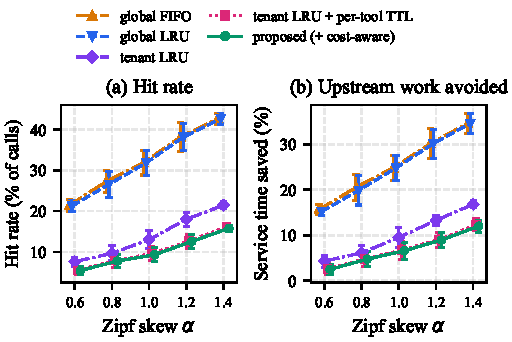
\includegraphics[width=\columnwidth]{figures/fig5_cache.pdf}
\caption{Cache policies versus Zipf skew $\alpha$ (four tenants, five trials; points offset horizontally for legibility): (a) hit rate and (b) share of upstream service time avoided. Leak and stale rates at $\alpha = 1.0$ are in Table~\ref{tab:cache}.}
\label{fig:cache}
\end{figure}

Fig.~\ref{fig:cache} and Table~\ref{tab:cache} compare six policies at equal capacity. Unscoped caches (global FIFO and LRU) have the highest hit rates because one tenant's result is reused for all, which is exactly the failure: at $\alpha = 1.0$, \cGlruLeak\% of \emph{all} calls under global LRU are answered with another tenant's data (\cGlruLeakHi\% at $\alpha = \cAlphaHi$), and \cGlruStale\% with data older than the tool's freshness bound, because one static TTL applies to every tool. Scoping keys by tenant eliminates leaks and lowers the hit rate from \cGlruHit\% to \cTlruHit\%, and per-tool TTLs eliminate the remaining \cTlruStale\% stale responses and lower it further; an unscoped cache's extra hits are precisely the responses it must not serve. Cost-aware eviction changes little at this capacity. The proposed cache reduces mean latency by \cPropLatGain\% on the single host (\cPropLat\ versus \cNoneLat\ms) and by \awCPropLatGain\% on EC2 (\awCPropLat\ versus \awCNoneLat\ms); hit, leak, and stale rates depend only on the trace and are identical on both. The saving grows with tool latency: with tools of about 100\ms, it is \hCPropLatGain\% of mean latency, or \hCPropSavedMs\ms per call.

\emph{When does cost-aware eviction pay off?} Over a grid fixed in advance (capacities of \senCapS, \senCapM, and \senCapB\ entries; tool costs of \senCurLo--\senCurHi\ms, 10--300\ms, and 10\ms--2\,s; \senSeeds\ paired traces of \senTrace\ calls at $\alpha = 1.0$), we compared the share of cacheable-tool service time avoided by the proposed policy and by tenant LRU with per-tool TTL. At \senCapS\ entries, cost-aware eviction avoids \senGainCur, \senGainMod, and \senGainWide\ percentage points more as the spread widens (\senPCur, \senPMod, and \senPWide), at up to \senHitLoss\ points lower hit rate; at \senCapM\ entries it avoids \senLossMin--\senLossMax\ points less, and at \senCapB\ entries nothing is evicted. Against a Bonferroni threshold of \senBonf, the gains at the two wider spreads and the loss at \senCapM\ entries with the emulation's costs remain significant. Cost-aware eviction thus pays off only when the cache is small relative to the working set and tool costs differ widely.

\subsection{Concurrency and Model Validation}
\label{sec:res-concurrency}

\begin{table*}[t]
\centering
\caption{Asymptotic-bound model versus measurement for $N \in \{1,\dots,128\}$ closed-loop sessions at 2 ms RTT, pool size $c = 16$. $R_1$ and $S_{\mathrm{hold}}$ are measured at $N=1$; $D_{\mathrm{cpu}}$ is measured CPU time per call at $N=1$ and at $N=128$. Errors are mean absolute percentage errors (MAPE) of the model using $D_{\mathrm{cpu}}$ at $N=1$ / at $N=128$.}
\label{tab:model}
\begin{tabular}{l rr rr c r r rr}
\toprule
 & $R_1$ & $S_{\mathrm{hold}}$ & \multicolumn{2}{c}{$D_{\mathrm{cpu}}$ (ms)} & Bottle- & Knee & Max $X$ & \multicolumn{2}{c}{MAPE (\%)} \\
\cmidrule(lr){4-5}\cmidrule(lr){9-10}
Transport & (ms) & (ms) & $N{=}1$ & $N{=}128$ & neck & $N^*$ & (calls/s) & throughput & latency \\
\midrule
T2 HTTP+SSE & 10.36 & 3.41 & 1.367 & 0.351 & cpu & 30 & 2392 & 33 / 9 & 101 / 7 \\
T3 unpooled & 16.23 & 15.53 & 2.604 & 0.757 & pool & 17 & 890 & 31 / 10 & 68 / 7 \\
T4 pooled & 10.40 & 9.73 & 1.025 & 0.423 & pool & 17 & 1451 & 15 / 8 & 24 / 6 \\
T4 + cache & 9.40 & 9.97 & 1.123 & 0.422 & pool & 15 & 1578 & 21 / 6 & 37 / 4 \\
\bottomrule
\end{tabular}
\end{table*}


\begin{figure}[t]
\centering
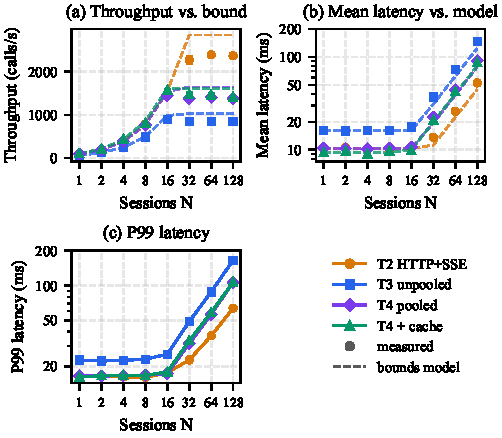
\includegraphics[width=\columnwidth]{figures/fig4_concurrency.pdf}
\caption{Closed-loop concurrency sweep at \qRtt\ms RTT with $c = \qPool$ connections (three trials): (a) throughput, measured (markers) and asymptotic bound (dashed); (b) mean latency, measured and model; (c) P99 latency. Dashed lines are model predictions from measured inputs, not fitted curves; the throughput bound is an upper limit.}
\label{fig:concurrency}
\end{figure}

\begin{table}[t]
\centering
\caption{Closed-loop results on Amazon EC2. $X_{\max}$ is the highest throughput over $N = 1$--128 sessions (three trials); P99 is T4's tail latency at the largest $N$. MAPE is the bounds model's throughput error across the four configurations, with $D_{\mathrm{cpu}}$ measured at the largest $N$ (load) or at $N = 1$.}
\label{tab:aws-throughput}
\footnotesize
\setlength{\tabcolsep}{2.1pt}
\begin{tabular}{ll r rrr r rr}
\toprule
 & & & \multicolumn{3}{c}{$X_{\max}$ (calls/s)} & T4 P99 & \multicolumn{2}{c}{MAPE (\%)} \\
\cmidrule(lr){4-6}\cmidrule(lr){8-9}
Placement & Security & RTT (ms) & T2 & T3 & T4 & (ms) & load & $N{=}1$ \\
\midrule
Same AZ & TCP & 0.15 & 4884 & 2203 & 2508 & 62 & 3--5 & 3--24 \\
 & TLS & 0.15 & 4552 & 815 & 2496 & 63 & 2--4 & 4--27 \\
\addlinespace
Cross AZ & TCP & 0.53 & 4619 & 2061 & 2366 & 65 & 3--4 & 11--31 \\
 & TLS & 0.54 & 4289 & 769 & 2320 & 66 & 3--4 & 17--33 \\
\addlinespace
Cross region & TCP & 12.73 & 1248 & 513 & 857 & 159 & 0--5 & 0--5 \\
 & TLS & 12.90 & 1254 & 347 & 825 & 166 & 1--5 & 1--5 \\
\bottomrule
\end{tabular}
\end{table}


\emph{Single host.} Fig.~\ref{fig:concurrency} and Table~\ref{tab:model} show $N = 1$ to 128 sessions and two regimes. Both Streamable HTTP transports are bounded by the pool ($c = \qPool$): T3 holds each connection for two emulated handshake RTTs plus the call and saturates at \qTthreeXmax\ calls/s (bound $c/S_{\mathrm{hold}} = \qTthreeBound$), and T4 holds it only for the call and saturates at \qTfourXmax\ calls/s (bound \qTfourBound), \qTfourOverTthree$\times$ T3. T2 is not pool-bound, because the POST connection is released after the 202 acknowledgment; it is limited by the single event loop and reaches \qTtwoXmax\ calls/s (CPU bound \qTtwoCpuBound), \qTtwoOverTthree$\times$ T3. Beyond saturation, latency grows linearly with $N$, as Little's law predicts (at $N = 128$, T4's P99 is \qTfourPnnmax\ms against \qTtwoPnnmax\ms for T2). The cache adds only \qTcacheGain\% to T4's saturation throughput, because its hit rate falls from \qTcacheHitOne\% at $N = 1$ to \qTcacheHitMax\% at $N = 128$: identical calls arriving together all miss, since the gateway does not merge concurrent identical requests. Peak traced heap growth is at most \qHeapMaxAll\,MB at $N = 128$.

\emph{EC2.} Table~\ref{tab:aws-throughput} repeats the sweep on separate instances, and the regimes reproduce. Within a region, T4 saturates near its pool bound and CPU-bound T2 sustains \awTtwoOverTfourInMin--\awTtwoOverTfourInMax$\times$ T4's throughput. Across regions, T2's submission connections, each held for a round trip until the 202 acknowledgment, become its bottleneck, and its advantage shrinks to \awTtwoOverTfourXXreg$\times$. \emph{Per-call TLS is a capacity problem even where latency is negligible:} in the same zone, a handshake per call raises T3's CPU time per call at $N = 1$ from \awCpuTthree\ to \awTlsCpuTthree\ms, moves its bottleneck from the pool to the CPU, and lowers its saturation throughput from \awTthreeXSame\ to \awTthreeXSameTls\ calls/s, while pooled T4 is unaffected (\awTfourXSame\ versus \awTfourXSameTls).

\emph{Model accuracy.} With $D_{\mathrm{cpu}}$ measured at the largest $N$, throughput MAPE is \qMapeXMin--\qMapeXMax\% on the single host and \awMapeMin--\awMapeMax\% on EC2, and latency MAPE \qMapeRMin--\qMapeRMax\% and \awMapeRMin--\awMapeRMax\%. With $D_{\mathrm{cpu}}$ measured at $N = 1$, throughput MAPE rises to \qMapeXOneMin--\qMapeXOneMax\% and \awMapeOneMin--\awMapeOneMax\%, largest for CPU-bound T2, because CPU time per call falls with load (T4: \qTfourDcpuone\ms at $N = 1$, \qTfourDcpumax\ms at $N = 128$) as per-wake-up cost is amortized over more ready events. Measured saturation throughput is \qBoundFracMin--\qBoundFracMax\% of the bound on the single host, where the upstream server shares the machine, and \awBoundFracMin--\awBoundFracMax\% on EC2 (up to \awBoundFracCacheMax\% with the cache, since hits need no connection). With tools of about 100\ms, single-host throughput MAPE is \hMapeMin--\hMapeMax\% with CPU time measured under load and at most \hMapeOneMax\% from single-session measurements.

\subsection{Deployment Cost}
\label{sec:res-cost}

\begin{figure}[t]
\centering
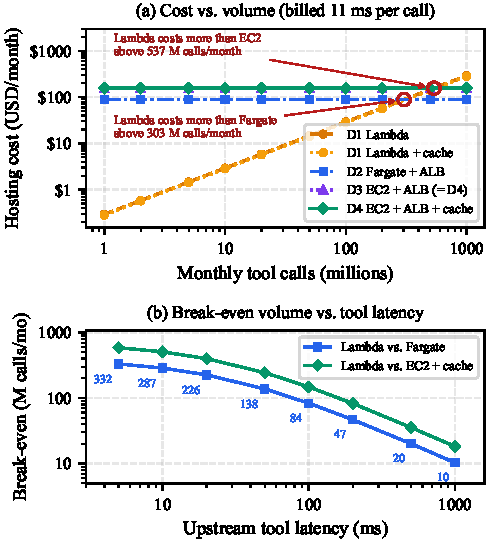
\includegraphics[width=\columnwidth]{figures/fig6_cost.pdf}
\caption{(a) Monthly gateway hosting cost versus call volume for serverless (Lambda), container (Fargate), and VM (EC2) deployments, from Eqs.~\eqref{eq:lambda}--\eqref{eq:vm} with measured inputs. (b) Break-even volume between Lambda and each always-on deployment as a function of upstream tool latency.}
\label{fig:cost}
\end{figure}

We instantiate Eqs.~\eqref{eq:lambda}--\eqref{eq:vm} with AWS on-demand list prices for us-east-1 (Lambda at \$0.20 per million requests and \$0.0000166667 per GB-s with 512\,MB; Fargate tasks of 1 vCPU and 2\,GB at \$\kFargate\ per month; m6i.large instances of 2 vCPUs at \$\kEcTwo\ per month; an application load balancer at \$\kAlb\ per month, excluding capacity-unit charges; at least two replicas; \kUtil\% target utilization). The measured inputs are the billed duration of a T4 call at 2\ms RTT (\kBilled\ms) and the CPU time per call at 32 sessions (\kCpuUnc\ms uncached, \kCpuC\ms cached). One vCPU then sustains about \kCapVcpu\ billion calls per month at the target utilization, so the always-on deployments stay at their two-replica minimum (\$\kFargateMin\ per month for Fargate and \$\kEcTwoMin\ for EC2, including the load balancer) across Fig.~\ref{fig:cost}(a), using about \kVcpuShareThousand\% of one vCPU even at a billion calls per month. Serverless is cheaper below about \kBreakevenFg\ million calls per month than Fargate and below about \kBreakeven\ million than EC2. A cache hit still requires authentication, authorization, and request inspection, so CPU time per call falls only slightly (about \kHitAtThirtyTwo\% of calls hit at 32 sessions); the cache's value lies in avoided upstream calls, not hosting cost. 
The break-even point is sensitive to tool latency because Lambda bills for the time a function waits on the tool. Holding the gateway-side time (\kGwSide\ms) fixed, the break-even volume against Fargate falls from \kBeFgTen\ million calls per month for 10\ms tools to \kBeFgHundred\ million for 100\ms and \kBeFgThousand\ million for 1\,s tools, and against EC2 from \kBeTen\ to \kBeHundred\ and \kBeThousand\ million (Fig.~\ref{fig:cost}(b)). Measuring with tools of about 100\ms (billed \hBilled\ms per call) gives \hBreakevenFg\ and \hBreakeven\ million, matching the model's \kBeFgHundred\ and \kBeHundred. For enterprise tools that take hundreds of milliseconds, per-invocation billing thus loses at modest volumes; platforms that bill only active CPU time would need separate modeling. With the billed duration and CPU time measured on EC2 (\awBilled\ms and \awCpuUnc\ms per call), the break-even volumes are about \awBreakevenFg\ and \awBreakeven\ million, so the conclusion does not depend on the desktop testbed.

% =====================================================================================
\section{Discussion}
\label{sec:discussion}

\subsection{Design Guidance}
\emph{Pool upstream connections}, sized to the offered concurrency ($c \gtrsim X \cdot S_{\mathrm{hold}}$) and served in arrival order; Streamable HTTP then needs no per-session state. \emph{Never pay a TLS handshake per call}. \emph{Rely on deterministic controls for safety}: identity, delegation, and per-tool authorization check credentials and policy rather than wording, and signature inspection is a filter for known indicators, not the safety boundary. \emph{Budget inspection by payload size} and use linear-time matching. \emph{Never share cached results across tenants or beyond tool-specific freshness bounds}: the hit rate lost to scoping is the hit rate that would have leaked. \emph{Merge concurrent identical calls} before relying on a cache under load. \emph{Size by CPU time measured at the operating load}, with one event loop per core or a compiled data plane once the pool is not the bottleneck, \emph{and model serverless cost with tool latency included}.

\subsection{Threats to Validity}
\emph{Network and placement.} The single-host experiments share one machine and emulate network delay at the application layer. The EC2 runs remove this limitation for the transport and concurrency experiments, but cover one instance type, three placements in two adjacent regions, and a single gateway process; they do not exercise packet loss, congested links, load balancers between agent and gateway, or multi-replica gateways. The cache, middleware, and security experiments are host-local by design and were repeated on EC2 only in the same zone.
\emph{Emulated service time.} Upstream tools sleep for an emulated service time, 2.1--10.5\ms in the main experiments and about 100\ms in the repeated ones, and return fixed payloads. The repeated runs confirm that slower tools shrink the relative transport overhead and raise the absolute value of caching and the cost of serverless billing, but real tools are also more variable, and no real MCP server was measured.
\emph{Implementation language.} The prototype is single-threaded Python. Absolute throughput would be higher in a compiled data plane. We expect the relative findings on handshake cost, linear inspection scaling, and cache trade-offs to carry over, but two results are specific to the implementation: the worst-case inspection stall arises from Python's backtracking regular-expression engine, which linear-time engines avoid, and T2's CPU bound reflects a single event loop.
\emph{Security suite.} Our own suite is small and authored by us. The public datasets are written by others but test the rules on text alone, not through an agent, so neither estimates how often an agent would be compromised in practice; agent-level benchmarks~\cite{debenedetti2024agentdojo,yang2025mcpsecbench} and learned detectors are not evaluated.
\emph{Workload.} Traces are synthetic with Zipf-distributed arguments; cache results depend on the reuse in real agent traffic, which has not been characterized publicly. Concurrent sessions issue calls with no pause between them, which maximizes how often identical calls arrive together, so the fall in hit rate under concurrency is closer to a worst case. We test one pool size ($c = \qPool$), four tenants, and list prices in one region.
\emph{Model validation.} The more accurate variant of the bounds model takes $D_{\mathrm{cpu}}$ from the same runs whose throughput it predicts (Section~\ref{sec:model}), so its error measures how well the bound's structure fits rather than how well it predicts from independent measurements; the variant using single-session measurements gives that estimate.
\emph{Staleness metric.} Staleness is defined relative to the per-tool freshness bounds that the proposed cache also enforces, so its zero staleness holds by construction; the measurement quantifies how often policies without those bounds violate them.

% =====================================================================================
\section{Conclusion}
\label{sec:conclusion}

We measured what the transport, security, caching, and deployment choices of an MCP gateway cost on one host and on Amazon EC2. On real networks transport dominates, and per-call TLS more than halves an unpooled gateway's capacity even within one zone. Deterministic identity and authorization controls cost about a tenth of a millisecond and cannot be evaded by rewording, whereas signature inspection is the only stage whose cost grows with payload size and detects none of \extAttacks\ public attacks. Correct caching costs hit rate, and concurrency erodes it further. A simple queueing bound predicts capacity to within \awMapeMin--\awMapeMax\% on EC2, and serverless billing is cheaper than two always-on replicas only below about \kBreakevenFg\ million calls per month for our short tools and \kBeFgHundred\ million for 100\ms tools. Future work will cover multi-replica gateways and lossy links, compare learned detectors on agent-level benchmarks, and characterize tool-call reuse in production traffic.

\section*{Data Availability}
The gateway prototype, benchmark harness, raw results, and scripts that generate every table and figure in this paper will be released upon publication.

\section*{Acknowledgment}
During the preparation of this work the authors used AI assistants (Claude, Anthropic~\cite{anthropic2026claude}; Gemini, Google~\cite{google2026gemini}; and Grok, xAI~\cite{xai2026grok}) to help write and debug the gateway prototype, the benchmark harness, and the scripts that generate the tables and figures, to help draft and edit the text of all sections, and to review drafts of the manuscript. The authors designed the study, reviewed and verified all code, results, and text, and take full responsibility for the content of this article.

\bibliographystyle{IEEEtran}
\bibliography{references}

\newpage
\begin{IEEEbiographynophoto}{He Li}
received the M.Eng. degree in computer science from Cornell University, Ithaca, NY, USA. He currently works as a software engineer in industry. His research interests include AI infrastructure, in particular the performance, security, and cost of systems that serve and connect large language model agents.
\end{IEEEbiographynophoto}

\begin{IEEEbiographynophoto}{Yi Zhong}
received the M.S. degree in computer science from Columbia University, New York, NY, USA. He currently works as a software engineer in industry. His research interests include AI infrastructure, in particular the performance, security, and cost of systems that serve and connect large language model agents.
\end{IEEEbiographynophoto}

\EOD
\vspace*{0pt plus 1filll}

\end{document}
